\documentclass{article}

\usepackage{pdfpages}
\usepackage{graphicx}

\usepackage{float}

\usepackage{adjustbox}
\usepackage{hyperref}

\usepackage{biblatex}
\addbibresource{references.bib}

\graphicspath{ {./images/} }

\title{
    \vspace{-4.0cm}
    {\Huge Social Routing}\\[0.5cm]    
    \textsc{\Large Project and Seminar}\\[0.5cm]
    \textsc{\large Instituto Superior de Engenharia de Lisboa}\\[0.5cm]
}

\date{\today}
\author{   
    \begin{minipage}{0.4\textwidth}
        \begin{flushleft} \large
        \emph{Authors:}\\
        Baltasar Brito\\
        {\small email: baltasar.brito@gmail.com}\\
        {\small phone: 915953552}\\
        Bernardo Costa\\
        {\small email: bjmcosta97@gmail.com}\\
        {\small phone: 913897555}\\
        \end{flushleft}
    \end{minipage}
    ~
    \begin{minipage}{0.4\textwidth}
        \begin{flushright} \large
        \emph{Supervisor:} \\ 
        Pedro Félix\\
        {\small email: pedrofelix@cc.isel.ipl.pt}\\  
        \end{flushright}
    \end{minipage}\\[2cm]  
}

\begin{document}     
    
    \maketitle

    \newpage

    \tableofcontents

    \newpage

    \section{Introduction}
    
        \subsection*{Report Structure}
        The structure of the report is based on the previously made timeline. Each of the timeline's points is explained and evaluated with regards to it's completion and difficulties that were overcome in it's implementation.\par
        The previously made timeline had incorrect delivery dates and as such this report will also present a correct and improved version of the future timeline to follow as well as the risks it might contain.
    
        \newpage
    
    \section{System Structure}
        \begin{figure}[h]            
            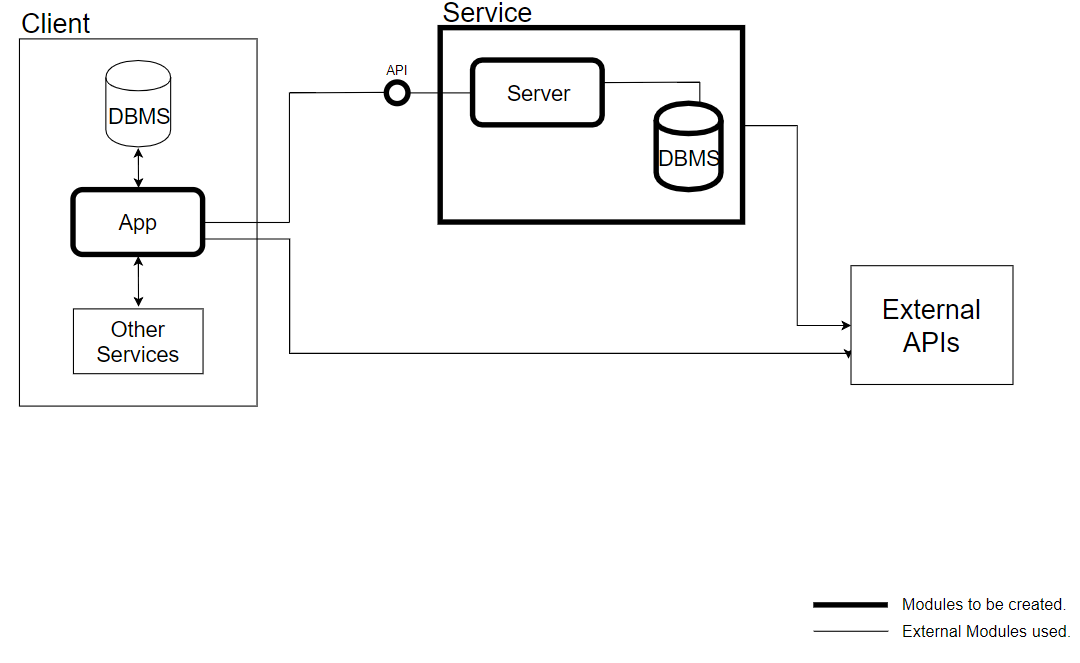
\includegraphics[width=\textwidth]{images/project-structure/system-structure.PNG}
            \caption{System structure.}
            \label{fig:systemstructure}
        \end{figure}  
        \newpage

    \section{Client Application}
        \subsection*{Infrastructure Design}

        \subsection*{Route Creation}

        \subsection*{Communication with the Social Routing API}

        \newpage

    \section{Social Routing Service}

        The Social Routing Service is responsible for providing access to data and functionalities to a client through an an HTTP \cite{httponlinedocs} based API. It receives HTTP made requests
        with certain specifications and responds with resources generated by the the server. The following diagram details the building blocks of the service:

        \begin{figure}[h]            
            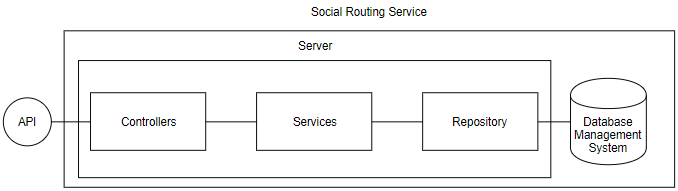
\includegraphics[width=\textwidth]{images/project-structure/service-structure.PNG}
            \caption{Social Routing Service structure.}
        \end{figure}  

        \subsection{Social Routing API}          
           
            The goal of the Social Routing API is to expose the service's functionalities to a client, in this case the an Android\cite{androiddocs} based client application. The API
            should be used to store or retrieve routes and user information, as well as to find the closest route available to a specific user or location.\par
            It was built in the Kotlin \cite{kotlinwebsite} programming language and using the {Spring MVC framework} \cite{springwebsite}. The build system is that of the server,
            which they both share with the framework itself, Gradle \cite{gradlewebsite}. \par 
            All API access is done over Hypertext Transfer Protocol and the API data is sent and received in the JSON \cite{jsonwebsite} format. The exception is on error responses
            which follows the JSON+problem \cite{jsonproblemonlinedocs} standard. \par
            Currently the API supports requests in a limited number of HTTP \textit{verbs} (GET, POST, PUT, DELETE) \cite{apihttpverbsdocs}, and has a functional but incomplete error handling system. 
            Some request specifications are already complete, such as the media type desired in a POST request but some are not such as user authentication. 

            \subsubsection*{Endpoint for Route Creation}
            The first task when building the API was to provide a way for a Route to be created because of the considerations it requires. Namely, the 
            characterization of a Route in it's data form and the metadata it needs in order to be stored and retrieved.\par
            
            This goal was achieved with success \cite{routecreationdocs} but with some minor problems in the characterization aspect occurring from time to time. 
            Initially a route was characterized by a set of coordinate pairs, that each had the latitude and longitude of a given geographic point, but 
            as the project grew the metadata required to characterize a route grew with it. At this time, for a route to be created it requires not only the 
            set of coordinates but also its creator's information and its assigned categories.

            \subsubsection*{Finalization}
            After the the API's structure was complete with the creation of a route the rest of the endpoints were added and are now functioning properly \cite{apidocs}.
            There are some functionalities left that will only be complete later on, like user authentication and error handling, the last one being now done 
            but in an incomplete albeit functional way.

            When adding each of the endpoints to the API the difficulty relied in a separation of concerns and requirements of both the server side and client side modules.
        
            \newpage
        
        \subsection{Server}    
            The role of the server within the system is to receive data, transform it, and either store it or process it and return it as a response. The technologies
            it requires to function are the same as the API.\par
            The \textit{flow} of an HTTP request that arrives on the server goes through the following pipeline: a Controller is assigned to a specific endpoint which will then
            use at least one service. If the request requires stored data the service will request it from a repository, if not, the service processes the data and returns 
            it in the correct form back to the controller which responds to the request with a response in a well defined format, depending on the request made. 

            \subsubsection*{Communication with the Database Management System}
            Initially the communication with the database was made using Spring Data JPA \cite{springjpadocs} but after the initial implementation with it, it revealed 
            itself to be time consuming on the learning side, and limited in the management of the database connection and SQL queries desired. That caused a switch to a different approach, using JDBI \cite{jdbidocs}.
            JDBI \cite{jdbidocs} is an API which is built on top of the JDBC driver \cite{jdbcdocs}.\par and is used directly in the server by the Repository component to communicate with the database.        

            \subsubsection*{Infrastructure Design and Implementation}
            The structure of the server follows the one showed in figure \ref{fig:systemstructure}. 
            Two Controllers were built, one for user related requests and other for route related ones. Following the diagram, the services follow the same logic, one for route related 
            processing and other one for user processing. The final layer is the repositories which depends directly on the entities present on the database. There are two repositories as well,
            one for user related operations and another for those that are route related.\par
            An also very important part of the server is also the conversion of data. Currently, a received request is transformed from received data in the JSON format to an input type object which is received by a controller, then to a data 
            transfer object and sent to one or multiple services and after that to a domain object which might be sent to a repository if database storage or retrieval is necessary.

            Setting this goal so early in the timeline allowed us to establish a foundation to build on top of in a very quick fashion, being that most of the work was done decided initially the rest 
            was just a question of adding an extra Repository, Service or Controller as well as the required type converters. 

            \subsubsection*{Add All Functionalities Except Search}
            The functionalities of the server required in this point were all the ones considered to support a functional API and as such, after the initial structure was done, most of the requirements
            that followed were a matter of adding and extra component horizontally being that the vertical structure was already complete. As far as the search functionality goes, it is implemented in 
            a minimalistic version, allowing for rout searching by location only.

            \newpage

        \subsection{Database Management System}
            The database management system chosen was PostgreSQL \cite{postgresql}, using the hybrid functionality of storing valid JSON directly in a table field \cite{postgresqljson}. The database is used to store
            all entities required for the service to function and to deliver them to repositories in need. 
            The decision of choosing JSON as a type to store data comes with the need of storing large sets of coordinates belonging to a single entity, this will allow us to 
            make faster and easier calculations of times and distances between routes and points rather than if a Point was it's own entity. 

            The following entity diagram represents the structure of the database:
            \begin{figure}[h]            
                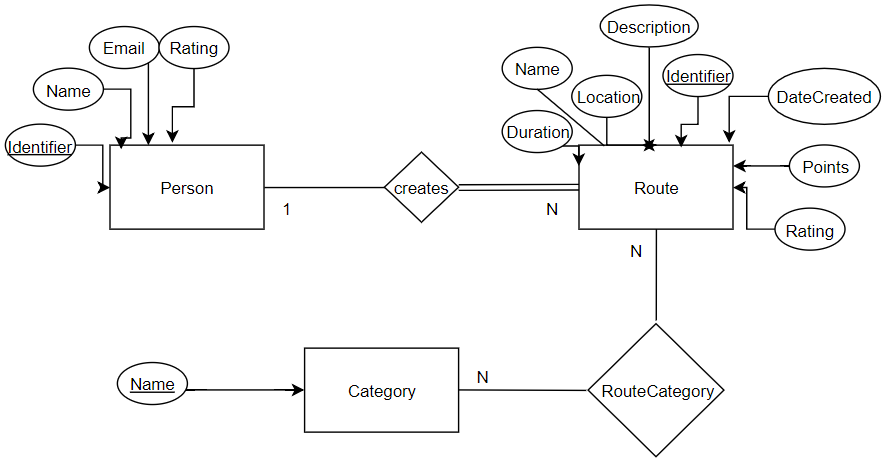
\includegraphics[width=\textwidth]{images/project-structure/dbms-structure.PNG}
                \caption{Entity Relationship Diagram.}
            \end{figure}  

            \subsubsection*{Route Saving}
            Route saving, like the first points of each other component, was chosen to be able to have a well defined structure of the whole project as quickly as 
            possible with the goals of structure first, implementations later. After characterizing a route \cite{dbmsroutecharacterization} the project had a fully functional minimalistic structure.

            \subsubsection*{Remaining Entities}
            After the initial structure was built the remaining entities were added to the database as needed. To maintain integrity and consistency of the data functions were added to support more complete queries that manipulate multiple tables.
            When inserting a route for example, the route has to reference at least one category, and as such an insert to the route table has to guarantee an insert to the RouteCategory table. The procedures are called by the repositories and executed by the database.

            \newpage
        
    \section{Updated Timeline}
        \begin{figure}[H]
            \begin{adjustbox}{addcode={
                \begin{minipage}{\width}}{
                    \caption{Updated timeline.}
                    \label{fig:updatedTimeline}
                \end{minipage}},rotate=90,center}
            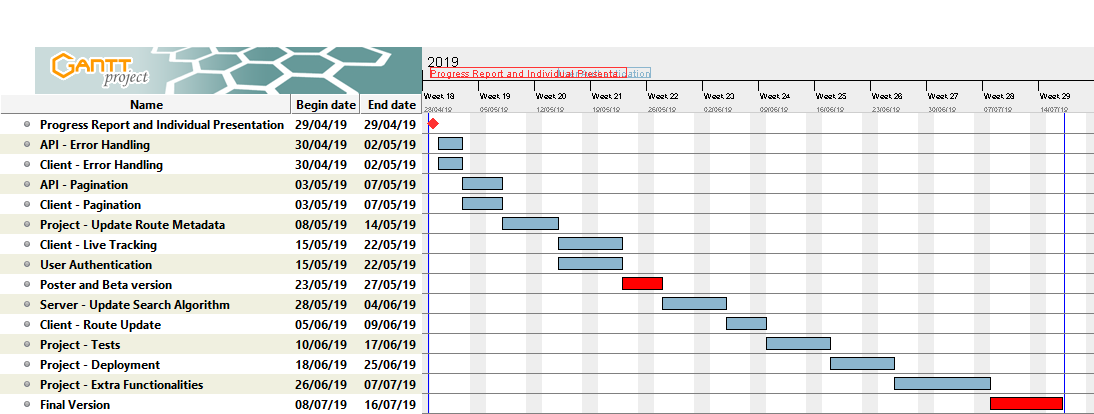
\includegraphics[width=0.9\textheight]{images/timeline/updatedTimeline.PNG}
            \end{adjustbox}
        \end{figure}
        \newpage

    \section{Risks}

        The main risk while making this project is the time to complete it and the way to minimize this is a well thought plan of action, hence the restructuring of the original timeline.
        The following list of risks will help us manage the time left as well as give us an idea of were we stand in the long term planning.

        \begin{itemize}
            \item Search Algorithm: given search parameters each user should have the best possible route suggested to him.  
            \item User authentication: using an external service and integrate it with both the client application and the Social Routing Service.
            \item Live tracking: the user should be able to follow the route in real time, on his device.
            \item External APIs comprehension and usage might take more time than initially expected.
            \item Tests: testing each component correctly might involve using external unknown libraries and the time necessary to create them might not be enough. 
        \end{itemize}
    
        \newpage    
    
    \section{Conclusion}
    
        \newpage    
    
    \printbibliography



\end{document}
